\documentclass[a4paper, oneside]{book}
\usepackage[italian]{babel}
\usepackage[utf8]{inputenc}
\usepackage[a4paper,top=2.5cm,bottom=2.5cm,left=2cm,right=2cm]{geometry}
\usepackage{amssymb}
\usepackage{amsthm}
\usepackage{graphics}
\usepackage{amsfonts}
\usepackage{amsmath}
\usepackage{amstext}
\usepackage{engrec}
\usepackage{rotating}
\usepackage[safe,extra]{tipa}
\usepackage{multirow}
\usepackage{hyperref}
\usepackage{enumerate}
\usepackage{braket}
\usepackage{marginnote}
\usepackage{pgfplots}
\usepackage{cancel}
\usepackage{polynom}
\usepackage{booktabs}
\usepackage{enumitem}
\usepackage{algorithm}
\usepackage{algpseudocode}
\usepackage{framed}
\usepackage{pdfpages}
\usepackage{pgfplots}
\usepackage{fancyhdr}
\usepackage{caption}
\usepackage{subcaption}
\usepackage{setspace}
\usepackage{hyperref}
\pagestyle{fancy}
\fancyhead[L,RO]{\slshape \rightmark}
\fancyfoot[C]{\thepage}

\title{Data and Computational Biology}
\author{Tommaso Ferrario (\href{https://github.com/TommasoFerrario18}{@TommasoFerrario18})}
\date{Ottobre 2024}

\pgfplotsset{compat=1.13}

\begin{document}

\maketitle
\newtheorem{teorema}{Teorema}
\newtheorem{dimostrazione}{Dimostrazione}
\newtheorem{definition}{Definition}
\newtheorem{esempio}{Esempio}
\newtheorem{osservazione}{Osservazione}
\newtheorem{nota}{Nota}
\newtheorem{corollario}{Corollario}
\tableofcontents
\renewcommand{\chaptermark}[1]{
    \markboth{\chaptername
        \ \thechapter.\ #1}{}}
\renewcommand{\sectionmark}[1]{\markright{\thesection.\ #1}}

\chapter{Introduction}
In this course, we will study the principles of modeling and analysis biology
data using simulation and AI models.

In the field of biology, the scale size varies from the organism like tree passing
through tissues and arriving at the cellular level. So we are considering elements
with the size that varies from meters to micrometers.

In particular, we can distinguish two main groups of organisms: bacteria and eukaryotes.

All this organisms have in common that all have DNA as genetic material. The DNA
is a molecule that contains the information necessary to build and maintain an
organism.

We can describe the DNA as a sequence of nucleotides. The nucleotides are the
building blocks of DNA. The DNA is a double helix structure, and the nucleotides
are paired in a specific way. The nucleotides are \textit{adenine}, \textit{thymine},
\textit{cytosine}, and \textit{guanine}.

This nucleotides are paired in the following way: \textit{adenine} with \textit{thymine}
and \textit{cytosine} with \textit{guanine}. This help us to save up space because
they are always complementary.

A \textbf{gene} is a sequence of nucleotides that contains the information to
create a protein. While a \textbf{genome} is the complete set of genes of an organism.

\begin{figure}[!ht]
    \centering
    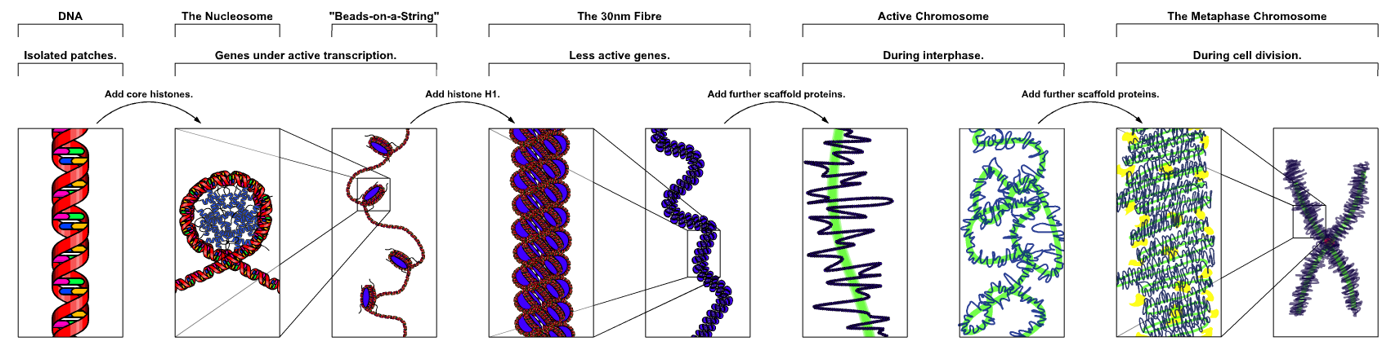
\includegraphics[width=\textwidth]{img/DNA.png}
    \caption{DNA structure}
    \label{fig:dna}
\end{figure}

A \textbf{genomic arm} refers to a large segment of a chromosome, typically
spanning several megabases (Mb) in size.

Starting from DNA we can create \textbf{RNA} through a process called \textbf{transcription}.
The RNA is a molecule that is used to create proteins. The proteins are the
building blocks of the cells. The process of creating proteins from RNA is called
\textbf{translation}.

The RNA transport information from nucleus, in other words, the DNA, to the
cytoplasm of a cell, where it mediates the process of translation to create proteins.

Once the information has passed into the protein it cannot get out again. The
transfer information from nucleic acid to nucleic acid, or from nucleic acid to
protein may be possible, but the transfer information from protein to protein,
or from protein to nucleic acid is impossible.
\section*{The Repressillator example}
A useful example to use as a base for the course is the repressillator. This is a
simple model of a genetic network that is able to oscillate. In particular, it is
compose of three proteins, $LacI$, $TetR$ and $\lambda CI$, that repress each other.

The structure of the repressillator is shown in Figure \ref{fig:repressillator}.
We can observe a circular structure, where each protein represses the next one in
the circle. This is a simple model of a genetic network that is able to oscillate.
More specifically, the LacI protein inhibits transcription of the second repressor
gene, TetR, which in turn inhibits the third repressor gene, $\lambda$ CI, which
in turn inhibits the first repressor gene, LacI.
\begin{figure}[!ht]
    \centering
    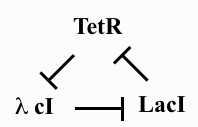
\includegraphics[width=0.5\textwidth]{img/repressillator.png}
    \caption{Structure of the repressillator.}
    \label{fig:repressillator}
\end{figure}

To implements this model, two \textbf{plasmids} are used. The plasmids are small
circular DNA molecules that are separate from the chromosomal DNA and can replicate
independently. The first plasmid codifies for the three proteins, while the second
plasmid serve as reporter of the system (GFP).

This system can be modeled using a set six of ordinary differential equations,
two for each protein. The general form of the equations is:
\begin{itemize}
    \item One equation for the variation of mRNA:
          \begin{equation}
              \frac{dM_i}{dt} = -m_i + \frac{\alpha}{1 + p_j^n} + \alpha_0
          \end{equation}
    \item One for representing the variation of the protein:
          \begin{equation}
              \frac{dP_i}{dt} = \beta (m_i - p_i)
          \end{equation}
\end{itemize}
where:
\begin{itemize}
    \item $\alpha$ is the proteins/cell from non repressed promoter.
    \item $\alpha_0$ is the proteins/cell from repressed promoter.
    \item $\beta$ protein mRNA decay velocity.
    \item $n$ Hill's coperativity coefficient.
\end{itemize}
\section{System, Biotech measures and Analysis}
During this course we want to measure two things:
\begin{itemize}
    \item \textbf{Gene expression}.
    \item \textbf{Gene alteration} also known as \textbf{mutation}.
\end{itemize}

The technology to obtain the information has evolved over time. In particular,
we have used \textit{microarrays} to measure gene expression, and now we use
\textit{next-generation sequencing} (NGS) for almost everything.

To collect data about gene expression, we can use \textbf{differential gene
    expression} (DGE). After using this approach, we can apply statistical
operation such as clustering or enrichment with genome ontology (GO).

With the enrichment phases we want to associate representative terms to the
clustering we have obtained. This operation is done in order to point out the
most important terms that are associated with the clustering.

\textbf{Gene ontology} is a controlled vocabulary that is use to describe gene.
It is divided in three categories:
\begin{itemize}
    \item \textbf{Biological process}: the biological objective to which the gene
          contributes.
    \item \textbf{Molecular function}: the biochemical activity of the gene product.
    \item \textbf{Cellular component}: the location of the gene product.
\end{itemize}
This information are express using a directed acyclic graph (DAG) where the main
type of association are \textbf{is a} and \textbf{part of}.
\subsection{Next-Generation Sequencing}
\textbf{Next-generation sequencing} (NGS) is a high-throughput methodology that
enables rapid sequencing of the base pairs in DNA or RNA samples.

The \textbf{sequencing} operation consists into fragmenting and extraction of
the DNA, then the DNA is sequenced and the \textbf{reads} are obtained. The reads
are short DNA fragments that are obtained from the sequencing process.

As computer scientists, we are interested in the dry-lab analysis which consists
in the \textbf{assembly} the \textit{reads} into a \textbf{Contigs}. Also, they
need to solve problem related to reads storage and allignments.

Talking about NGS, we can distinguish different approaches:
\begin{itemize}
    \item \textbf{Whole-genome sequencing} (WGS): the process of determining the
          complete DNA sequence of an organism's genome at a single time. This
          can be \textit{de novo} which mean that we don't have any reference
          genome.
    \item \textbf{Exome sequencing}: the process of capturing and sequencing the
          coding region of the genome.
    \item \textbf{Targeted sequencing}: the process of capturing and sequencing
          specific regions of the genome.
    \item \textbf{RNA sequencing} (RNA-Seq): the process of determining the
          complete RNA sequence of an organism's genome at a single time.
\end{itemize}

Also, talking about the analysis we can distinguish two types of analysis:
\begin{itemize}
    \item \textbf{Bulk analysis}: in this approach we use a pool of cells to analyze
          the gene expression. In particular, we create a average cell where we
          can study the overall gene expression.
    \item \textbf{Single cell analysis}: in this approach we analyze the gene
          expression of a single cell. This approach is more expensive and complex
          but it allows to study the gene expression of a single cell.
\end{itemize}
\subsection{From Sequencing to Mutational Information}
Thanks to the NGS we can obtain sequence that reveal different aspect of a
biological phenomenon. In this case, we can describe different subtypes of
mutations. Also, using bulk sequencing we can build a phylogeny tree that
describe the evolution of the mutation.
\chapter{Chemistry and Reactions}
\begin{definition}[\textbf{Mixture}]
    In chemistry the forms of matter are called \textbf{mixtures}. Some of them
    are \textbf{homogeneous} and others are \textbf{solution} with a \textbf{solvent}
    and a \textbf{solute}.

    To separate the components of a mixture we can use different methods like
    \textbf{filtration}, \textbf{distillation}, \textbf{chromatography} and
    \textbf{evaporation}.
\end{definition}
\begin{definition}[\textbf{Compound}]
    Certain substances are not separable by simple physical methods. These are
    called \textbf{compounds} and are formed by the union of two or more elements.
\end{definition}
\begin{definition}[\textbf{Reactions}]
    Pure substances cannot be further separated by means of physical interventions,
    but can be modified by means of (bio)chemical reactions.

    A reaction involves a certain number of reactants, yielding a number of products.
    \begin{equation}
        R_1 \bigoplus R_2 \bigoplus \ldots \bigoplus R_n \rightarrow P_1
        \bigoplus P_2 \bigoplus \ldots \bigoplus P_m
    \end{equation}

    As we all know, there are bits of matter that cannot be modified at the
    chemical level. These are called \textbf{elements}.
\end{definition}
\begin{definition}[\textbf{Atoms}]
    Atoms are composed by nuclei (protons and neutrons) and electrons on (quantized)
    orbits. Every orbit can contain up to 8 electrons (except for the first,
    which can hold only 2) this fact is known as the octect rule.

    The most external orbit is, except for the “noble gases”, incomplete; the
    number of electrons that occupy them determine the atom valence.
\end{definition}

The configuration of the external orbits of atoms, allows them to bind together
in compounds. Molecule structure depends on the organization of the electron
sharing in the most external orbits.

Atoms with valence up to 4 tend to be electron donors to atoms with a valence
from 5 to 7; atoms are therefore grouped in donors and receptors. Receptors atoms
are said to have an electronegative tendency.

There are several ways atoms bind to each other, the most common are:
\begin{itemize}
    \item \textbf{Ionic bindings} happen between atoms with very different valence.
    \item \textbf{Covalent bindings} happen between atoms of similar valence.
\end{itemize}

Molecules have a polarity, depending on the electronegativity of each participant
atom and their spatial configuration. Polar molecules tend to attract each other,
while non-polar molecules are relatively.

The forces that create bonds between atoms are also responsible of the attraction
between atoms and molecules. An intermediate attraction force is that resulting
from \textbf{hydrogen bonds} which keep together the DNA double helix.
\section{Reactions and Metabolism}
Biochemical reactions modify properties of various compounds and we can classify
them in two main categories:
\begin{itemize}
    \item \textbf{Reversible reactions} are those that can be reversed by changing
          the conditions of the system. They can be analyze at the equilibrium.
    \item \textbf{Irreversible reactions} are those that cannot be reversed.
\end{itemize}
The quantitative ratio among compounds in a reaction is called the reaction
\textbf{stoichiometry}.
The translation of stoichiometric ratios into physical quantities and vice-versa
requires the introduction of new units. So, chemists have defined the \textbf{mole}
as the quantity of substances comprising about $6.022 \times 10^{23}$ molecules.

This analysis is performed by looking at concentrations of a substance, measured
in mole/liter; this dimension is called the molarity of a solution.

Every reaction has its own reaction rate also called velocity. Given a reaction,
when the concentration of a reactant is very low, or the reaction rate is very
slow, then the reaction is said to be kinetically impaired.

A reaction can happen only when a positive $\Delta G$ is present and that is
enough to exceed the so-called activation barrier; such amount of energy is known
as activation energy.

Energy contained in ATP phosphate bonds is sufficient for the activation of
several biochemical reaction. This energy is however not enough to endanger several
of the other bond types that are present in an organism.

The metabolism is the activity that allows an organism to survive. This process
is mostly carried out in the cytoplasm of the cells and we can divide it in two
main categories:
\begin{itemize}
    \item \textbf{Catabolism} is the set of reactions that decompose various
          complexes, mostly acquired from the environment.
    \item \textbf{Anabolism} is the set of reactions that synthesize complexes.
\end{itemize}

Many of the basic reactions are shared, without much variation, by most living
organisms this is known as core metabolism. The metabolism that is specialized
for a class of organisms is dubbed secondary metabolism.

A very important process is the one that allows an organism to “load” ADP molecules
with a phosphate group, thus generating ATP. To obtain this result, organisms use
chains of reactions, called \textbf{metabolic pathways}.

Several of these reactions have a rather high activation energy or a quite slow
reaction rate. To speed up such reactions, organisms use the catalysis machinery.
A catalyzer speeds up a reaction or lowers its activation energy without being
consumed. Catalyzers are called enzymes, acting on substrates.
\section{Mathematical Modeling of Reactions}
Much of Computational Biology is \textbf{modeling reaction networks} which can be
subdivided in two main categories:
\begin{itemize}
    \item \textbf{Metabolic networks} are the set of reactions that take place
          in a cell. These reactions are mostly catalyzed by enzymes.
    \item \textbf{Regulatory networks} are the set of reactions that regulate
          the activity of the metabolic networks.
\end{itemize}
\subsection{Law of Mass-Action}
Collision between two chemical compounds $A$ and $B$ happen with a rate $k$ and
produce a compound $C$.
\begin{equation*}
    A + B \xrightarrow{k} C
\end{equation*}

We can rewrite the previous equation as:
\begin{equation}
    \frac{\delta [C]}{\delta t} = k [A][B]
\end{equation}
where with $[A]$ we denote the concentration of compound $A$. As said before,
we have also reaction that can be reversed, so we can write:
\begin{equation}
    A + B \mathrel{\mathop{\rightleftarrows}^{\mathrm{k_1}}_{\mathrm{k_2}}} C
\end{equation}
and the rate of the reaction is:
\begin{equation}
    \frac{\delta [A]}{\delta t} = k_2 [C] - k_1 [A][B]
\end{equation}
When a system is at equilibrium, the concentration don't change, therefore the
following condition holds:
\begin{equation}
    \frac{k_1}{k_2} = K_{eq} = \frac{[A]_{eq} [B]_{eq}}{[C]_{eq}}
\end{equation}
where $K_{eq}$ is the equilibrium constant of the reaction. If $K_{eq}$ is small,
then this is an indication that, at equilibrium, the concentration of $A$ and $B$
are effectively combined to form $C$.

Enzymatic reactions, which are non elementary reactions, can be modeled by the
Michaelis-Menten equation:
\begin{equation}
    S + E \mathrel{\mathop{\rightleftarrows}^{\mathrm{k_1}}_{\mathrm{k_2}}} catalysis \xrightarrow{k_3} P + E
\end{equation}
where $S$ is the substrate, $E$ is the enzyme, $P$ is the product and catalysis
and $C$ is the intermediate product.

Let's now consider the total enzyme concentration to be $[E]_0 = [E] + [C]$ and
also that all the reaction rate are constant. We can define the velocity at which
we increase the product concentration is:
\begin{equation}
    \frac{\delta [P]}{\delta t} = k_3 [C] \approx [E][S]
\end{equation}
so we can say that the velocity is proportional to the concentration of $[E]$ and
$[S]$.

The Michaelis-Menten system can be analytically solved by an equilibrium
approximation where we assume that the substrate $S$ and the complex $C$ are in
instantaneous equilibrium. This assumption allows us to write the following:
\begin{equation}
    k_1[S][E] = k_2[C] + k_3[C]
\end{equation}
Since $[E]_0 = [C] + [E]$, we can rewrite the previous equation as:
\begin{equation}
    [S][E]_0 - [S][C] = [C]\left( \frac{k_1 - k_3}{k_2}\right)
\end{equation}
We now introduce the Michaelis constant $K_M = \frac{k_2 + k_3}{k_1}$ which is
the combination of the rate constants of the reaction. We can rewrite the previous
equation as:
\begin{equation}
    [C] = \frac{[S][E]_0}{K_M + [S]}
\end{equation}
The velocity of the creation of $P$ is then:
\begin{equation}
    V = \frac{\delta [P]}{\delta t} = k_3[C]
\end{equation}
At $V_{max}$ we have that all the enzyme $E_0$ must be bound in the complex $C$,
this means that:
\begin{equation}
    V_{max} = k_3[E]_0
\end{equation}

If we now put everything together, we can write the Michaelis-Menten equation as:
\begin{equation}
    V = \frac{V_{max}[S]}{K_M + [S]}
\end{equation}
We can say that the Michaelis-Menten constant is a concentration ($\approx [S]$)
at which the velocity is half of $V_{max}$. In formula:
\begin{equation}
    V = \frac{V_{max}[S]}{K_M + [S]} = \frac{V_{max}}{2}
\end{equation}
\chapter{Computational Modeling}
\section{Deterministic Models}
We start by considering a deterministic model, which is a system of ordinary
differential equations (ODEs) that describe the time evolution of the
concentrations of the species in the system.

The main issue of deterministic models is \textbf{time}, which is represented
as a discrete variable.

The standard tool use to model deterministic models is the \textbf{ordinary
    differential equations} (ODEs). The ODEs are a set of equations that describe
the time evolution of the concentrations of the species in the system.

A different approach is to use \textbf{discrete event simulation} (DES), which
are a queue of events generated by a sources and processed by components. In this
representation, time is usually a derived notion, for example observing the
sequence of events.

\subsection{Stem Cell Differentiation}
The first model we consider is the stem cell differentiation model. The
\textbf{stem cell} differentiate into \textbf{progenitor cells}, which in turn
differentiate into \textbf{regular cells}.

The division or proliferation of stem cell can be:
\begin{itemize}
    \item \textbf{Symmetric}: the stem cell divides into two stem cells.
    \item \textbf{Asymmetric}: the stem cell divides into one stem cell and one regular cell.
    \item \textbf{Envirormentally Asymmetric}: the stem cell divides into one
          stem cell and one progenitor cell.
\end{itemize}

A first simple model of stem cell can be represented by a finite state machine
describe in Figure \ref{fig:stem_cell_fsm}.

\begin{figure}[!ht]
    \centering
    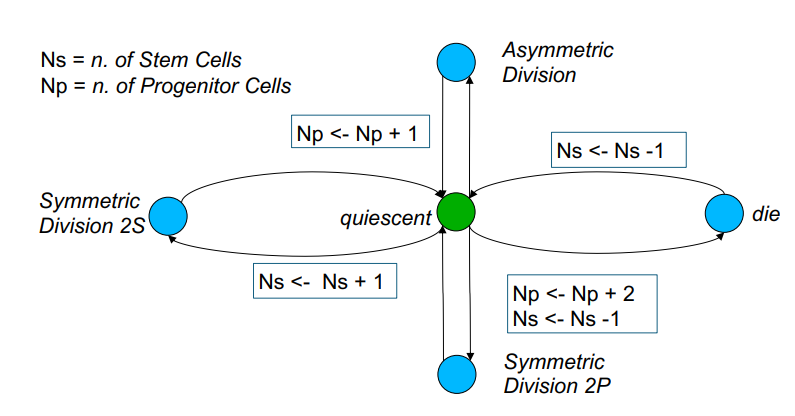
\includegraphics[width=.7\textwidth]{img/stemcellsFSA.png}
    \caption{Stem Cell Finite State Machine}
    \label{fig:stem_cell_fsm}
\end{figure}

In this example we don't consider the time. Time can be model considering an
exponential delay to the transition. Moreover, we can associate a different
probability to each transition, so we have a transition system (Markov Chain).
\section{Implementing a simulator}
In order to implement a simulator we need to define what means for us to run a
simulation. We can define a simulation as a sequence of events that can be
described by numerically solving a set of ODEs or by tracking the sequence of
events in a DES. This produce a \textbf{trace} of the simulation.

A trace is a sequence of vectors of values, where each vector represents the
state of the system at a given time. The trace can be used to analyze the
behavior of the system.

The engine of a simulator is essentially a loop where is body determines the
type of simulator we are using.
\subsection{Finite State Automata Simulator}
To implement a finite state automata simulator we need to define the following
elements:
\begin{itemize}
    \item \textbf{Specification}: first we need to define a set of finite
          automata, each represented by a matrix.
    \item \textbf{Engine}: check the set of all the enabled transitions from the
          current state and produce the next state.
    \item \textbf{Specification}: sources, computing units and sinks.
    \item \textbf{Trace}: a sequence of states.
\end{itemize}


\end{document}